\section{Evaluation}

Goals of the evaluation.
\begin{enumerate}
	\item Investigate practical applicability of RPQ evaluation by the proposed algorithm
	\item Compare Azimov's algorithm for reachability CFPQ and the proposed algorithm 
	\item Compare modified Azimov's algorithm for single-path CFPQ and the proposed algorithm 
\end{enumerate}

Hardware.

\subsection{RPQ}

In oder to do smthng....

Dataset description, tools selection.

\subsubsection{Dataset}

Dataset for evaluation

We evaluate our solution on RPQs 
We choose templates of the most popular RPQs which are presented in table~\ref{!!!}
We generate 10 queries for each template and each graph which randomly use relations from the given graph.

\subsubsection{Results}

Results of evaluation

Index creation.

\begin{figure}
   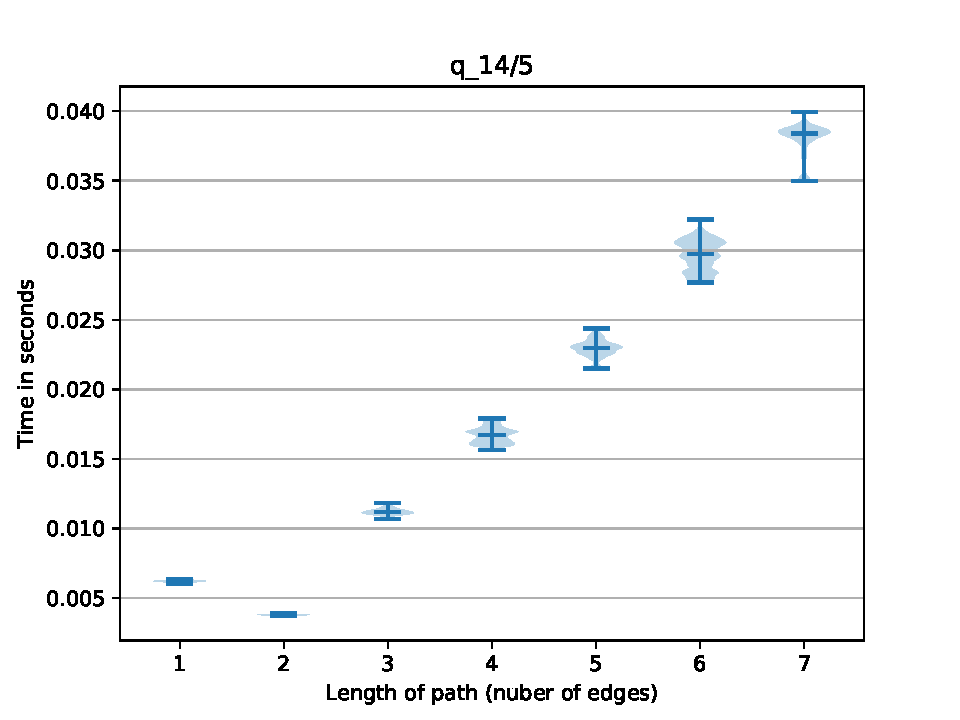
\includegraphics[width=0.48\textwidth]{data/res_graphics/q_14_5.pdf}
   \caption{Single path extraction}
\end{figure}

Paths extraction

\subsubsection{Conclusion}

\subsection{CFPQ}

Comparison with matrix-based algorithm.

\subsubsection{Dataset}

Dataset for evaluation. 
It should be CFPQ\_Data\footnote{CFPQ\_Data is a dataset for CFPQ evaluation which contains both synthetic and real-world data and queries \url{https://github.com/JetBrains-Research/CFPQ\_Data}. Access date: 07.07.2020.}

Same-generation queries, memory aliases.

\subsubsection{Results}

Results of evaluation.

Index creation.

Paths extraction.

\subsubsection{Conclusion}
